\chapter{Introduction}

\begin{figure}[!h]
\centering
            \subfloat[t=0]{
\includegraphics[width=.25\textwidth]{images/glider_gun/1.png}}\hfill
            \subfloat[t=10]{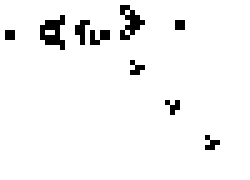
\includegraphics[width=.25\textwidth]{images/glider_gun/2.png}}\hfill
            \subfloat[t=20]{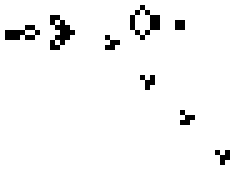
\includegraphics[width=.25\textwidth]{images/glider_gun/3.png}}\hfill
            \subfloat[t=30]{
\includegraphics[width=.25\textwidth]{images/glider_gun/1.png}}\hfill
            \caption{Gosper's Glider Gun, the first known pattern to exhibit unbounded growth in Conway's Game of Life.\cite{hickerson}}
\label{fig:gospers-glider}
\end{figure}

\section{Motivation}
Predicting effects is easier than predicting causes. This is the crux of the inverse problem in science. Causal opacity makes it easier to estimate observations from a parameterised model of the world than to recover parameters from observations. For instance, a physical model of the universe may allow us to predict the subatomic particles ejected when two protons collide at high speed but building theories based on such collisions is difficult, especially when there are multiple equally valid explanations. Despite this, the pursuit of inverse problems is critical to advancing scientific theory around a system's behaviour.\\

In this thesis, we tackle the inverse problem for cellular automata (CAs). These are simple yet powerful models of computation in which a discrete lattice of identical "cells" are simultaneously updated at regular time steps. The state of each cell depends exclusively on the state of the cells in a local neighbourhood around it in the previous time step. This localised interaction makes CAs a useful abstract representation for many physical and biological systems including tumor growth\cite{deutsch2021bio, reher2017cell}, urban land use\cite{white2000high}, and epidemics\cite{white2007modeling}. Like these systems, CAs can exhibit chaos, nonlinear dynamics, and the emergence of complexity. As well as simulatory models, CAs are powerful computational engines owing to their inherently parallel structure. This makes their study a useful endeavour in the field of distributed computation too\cite{tosic2005cellular}.\\


\section{Objectives}

Top-down investigations into CA behaviour are vast and varied\todo{cite}. Mathematical analyses seek to classify CAs and prove general results about long-term behaviour from intrisic properties. In the natural and social sciences, CAs are designed to model real world systems. In this thesis, we explore a bottom-up approach where we deduce the underlying properties of a CA by observing its behaviour. In particular, we use evolutionary algorithms to learn transition functions that define the behaviour of a CA.\\

Evolutionary algorithms (EAs) have long been held as effective tools for black-box optimisation problems. Grounded in the principles of Darwinian evolution, EAs traverse over a search space by performing selection, mutation, and crossover on a population of candidate solutions. As selection pressure grows, increasingly strong solutions emerge. Using EAs, we tackle multiple optimisation problems from procedural generation of desirable states to fully learning the dynamics of the system.\\

We focus on two classes of CA in particular. The first are binary outer-totalistic CA which are a discrete family of models in which Conway's infamous "Game of Life" CA belongs. For this reason, they are also called "life-like CA". The second are Gray-Scott models which simulate the behaviour of two diffusive chemicals. The three objectives of this project are:

\begin{enumerate}
    \item \textbf{Procedural generation}\label{obj-1}\\
    Use evolutionary algorithms to learn transition functions for life-like CA that induce stable states with desirable properties for random initial conditions.
    \item \textbf{Learning discrete CA dynamics}\label{obj-1}\\
    Use evolutionary algorithms to learn the exact transition function of life-like CA based on a small sample of observations.
    \item \textbf{Learning continuous CA dynamics}\\
    Use evolutionary algorithms to learn the exact transition function of Gray-Scott models based on a small sample of observations.
\end{enumerate}



\section{Contributions}
The technical contributions of this project are:
\begin{itemize}
    \item \textbf{Evolutionary algorithm toolkit}\\ A versatile toolkit that implements multiple evolutionary algorithms to train and optimise different classes of CA. We use this to predict the update rule of life-like CA from observations on random initial conditions. We show that this can be extended to Gray-Scott models where we predict the parameters of diffusion-reaction equations from simulations of chemical reactions.
    \item \textbf{Cellular automaton simulator}\\ A system that can efficiently simulate discrete and continuous cellular automata. This allows various fitness functions to be implemented in the EA toolkit. This can also render snapshots of the CA directly during simulation which allows animations to be automatically generated afterwards.
    \item \textbf{Procedural maze generator}\\ A CA-based maze generation program that uses the EA toolkit to produce "difficult" mazes. Mazes generated are guaranteed to have a solution and are optimised to exhibit characteristics preferred by users such as a long solution path and many dead ends.
    % \item \textbf{Systematic analysis of life-like CA}\\ An analysis of every life-like CA based on repeated finite time simulations over random initial conditions. This provides statistical support to previous mathematical analyses on 2D CA behaviour\todo{cite}.
\end{itemize}

\section{Technical Challenges}
The primary technical challenges faced during this project were:
\begin{itemize}
    \item \textbf{Ensuring efficient simulation}\\ Each evolutionary algorithm runs on large populations over multiple epochs. Fitness is calculated by repeated simulation of individual CAs which means that thousands of simulations need to be run for each experiment. Therefore, the simulator must be efficient. This is especially important for the Gray-Scott simulator which uses numerical integration to approximate solutions for the continuous differential equations that underlie chemical interactions.
    \item \textbf{Avoiding local optima}\\ Evolutionary algorithms are very susceptible premature convergence. We tackle this by using different types of evolutionary algorithm, testing a range of genetic operators, and designing creative loss functions.
    \item \textbf{Media generation}\\ Effectively learning from experiments requires statistical summaries, images, and animations to be produced. These provide quantitative and qualitative feedback for later analysis. Converting numerical data into high-fidelity media was a key point of focus.
\end{itemize}
